
\documentclass[11pt]{article}
    \usepackage{pdfpages} 
  	\usepackage{ucs} 
	\usepackage[utf8x]{inputenc} % Включаем поддержку UTF8  
	\usepackage[russian]{babel}  % Включаем пакет для поддержки русского языка 
	\usepackage {mathtext}
	\usepackage{amsmath, amssymb}
	\usepackage{graphicx}
	\usepackage{listings}
	\usepackage{hyperref}
	\usepackage{revsymb}
	\usepackage{listings}
\lstset{language=[90]Fortran,
  basicstyle=\ttfamily,
  keywordstyle=\color{red},
  commentstyle=\color{green},
  morecomment=[l]{!\ }% Comment only with space after !
}
	\hypersetup{
    colorlinks=true,
    linkcolor=blue,
    filecolor=magenta,      
    urlcolor=cyan,
	}
	\urlstyle{same}
	\DeclareGraphicsExtensions{.pdf,.png,.jpg,.jpeg}
	\setcounter{MaxMatrixCols}{20}
	\graphicspath{{pictures/}}
    \title{\textbf{Вычисление алгоритма Берштейн-Вазирани в Qiskit \\ -- \\ 
	Computing the Berstein-Vazirani algorithm in Qiskit}}
    \author{И.А.Юхновский}
    \date{ноябрь 2020}
    

\begin{document}
\maketitle
\thispagestyle{empty}
\section*{Аннотация}
В статье приведен практический пример использования фреймворка для квантовых вычислений на примере вычисления алгоритма Берштейн-Вазирани в Qiskit.


\section*{Abstract}
The article provides a practical example of using a framework for quantum computing using the example of computing the Berstein-Vazirani algorithm in Qiskit.

\section{Введение}
Qiskit - это платформа с открытым исходным кодом для работы с квантовыми компьютерами на уровне схем, импульсов и алгоритмов.

Основная цель Qiskit - создать программный стек, упрощающий использование квантовых компьютеров для всех. Однако Qiskit также стремится облегчить исследования по наиболее важным открытым вопросам, с которыми сегодня сталкиваются квантовые вычисления.

Продемонстрируем на практике как использовать Qiskit для реализации алгоритма Берштейн-Вазирани с возможностью запускать на симуляторах и реальных квантовых компьютерах. ~\cite{qiskit}

\section{Задача Бернштейна — Вазирани}
Алгоритм Бернштейна — Вазирани является расширенной версией алгоритма Дойча — Йожи (уже рассмотренный нами в предыдущей работе <<Теоретическое исследование возможности построения квантового компьютера на источниках ионизирующего излучения>>), поскольку вместо определения принадлежности функции к определённому классу — сбалансированная или постоянная (то есть принимает либо значение 0, либо 1 при любых аргументах) — алгоритм находит «спрятанный» вектор, позволяющий однозначно определить значение функции в любой точке ~cite{coles}.

Алгоритм Бернштейна — Вазирани демонстрирует в решаемой им задаче зазор между классическими и квантовыми алгоритмами по наименьшему требуемому количеству запросов к оракулу (чёрному ящику). Даже если разрешить использование вероятностных алгоритмов (с заранее ограниченной вероятностью ошибки), решение классической задачи потребует $O(n$ обращений к оракулу, в то время как в квантовом алгоритме достаточно $O(1)$ обращений к нему ~\cite{hidary}.

Далее рассмотрим постановку задачи и алгоритмы решения предложенные в ~\cite{coles}

\subsection{Классическая задача}
Пусть существует оракул, преобразующий $n-$битное число в один бит:

\begin{equation}
f:\{ 0, 1\}^n \rightarrow \{ 0, 1\}
\label{eq_1}
\end{equation}

такой, что:

\begin{equation}
f(x) = a \cdot x
\label{eq_2}
\end{equation}

, где $\cdot$ скалярное произведение вида $x \cdot y = x_1y_1 \oplus x_2y_2 \oplus \dots \oplus x_ny_n$.

Считаем, что один вызов функции $f$ осуществляется за константное время. Требуется найти $a$.

\subsection{Квантовая задача}
Постановка задачи в квантовой модели похожая, но доступ к оракулу в ней осуществляется не напрямую через функцию $f$, а через линейный оператор $U_f$, действующий на систему из $n+1$ кубита:

\begin{equation}
U_f = \sum\limits_{x \in \{0,1\}^n, y \in \{0,1\}} |x\rangle \langle x | \otimes | y \oplus f(x) \rangle \langle y |
\label{eq_3}
\end{equation}
, где: 
\begin{itemize} 
\item $|x \rangle $  — кет-вектор, соответствующий квантовому состоянию $x$, 
\item $\langle x|$ — бра-вектор, соответствующий квантовому состоянию $x$, 
\item $\otimes$  — произведение Кронекера, 
\item $\oplus$  — сложение по модулю 2.
\end{itemize} 

Квантовым состояниям $0$ и $1$ соответствуют векторы $|0\rangle =\binom {1}{0}$ и $|1\rangle =\binom {0}{1}$.
Вектор для совместного состояния $x_{1}x_{2}\dots x_{n}$ может быть представлен как произведение $|x_{1}x_{2} \dots x_{n} \rangle =|x_{1}\rangle \otimes |x_{2}\rangle \otimes \dots \otimes |x_{n}\rangle $.

Аналогично классическому случаю, предполагается, что обращение к оракулу, вычисляющему результат применения оператора $U_{f}$ к входящей системе из $n+1$ кубита, выполняется за константное время.

Предполагается, что:
\begin{equation}
f(x)=a\cdot x
\label{eq_31}
\end{equation}

 
 Требуется найти $a$.

\subsection{Алгоритм}
\subsubsection{Классическая задача}
В классическом случае при каждом вызове оракула возвращается один бит числа $a$, поэтому чтобы найти $n-$битное число $a$, нужно вызвать оракул $n$ раз. Ниже приведён вариант $n$ обращений к оракулу, позволяющих целиком восстановить $a$:

$f(1000...0_{n})=a_{1}$

$f(0100...0_{n})=a_{2}$

$ \vdots $

$f(0000...1_{n})=a_{n}$


Количество обращений к оракулу в классическом случае равно $O(n)$, где $n$  — количество бит числа $a$. Несложными теоретико-информационными рассуждениями можно показать, что эта оценка не улучшаема даже в рамках класса BPP ~\footnote{~\url{https://en.wikipedia.org/wiki/BPP_(complexity)}}.

\subsubsection{Квантовый алгоритм}
Определяется n-кубитный оператор Адамара:

\begin{equation}
H^{\otimes n} = \frac{1}{\sqrt{2^n}} \sum \limits_{x,y \in \{0,1\}^n}(-1)^{x \cdot y} | y \rangle \langle x|
\label{eq_4}
\end{equation}

и учитывается, что применение оператора $U_f$ к состоянию вида: 

\begin{equation}
|x\rangle |-\rangle = |x\rangle \otimes |-\rangle
\label{eq_5}
\end{equation}

, где 

\begin{equation}
|-\rangle = \frac{|0\rangle \otimes |-1\rangle}{\sqrt{2}}
\label{eq_6}
\end{equation}


дает в результате величину:

\begin{equation}
U_f(|x\rangle |-\rangle) = (-1)^{f(x)}|x\rangle |-\rangle
\label{eq_7}
\end{equation}

\subsubsection{Пошаговая работа алгоритма}
На первом шаге оператор Адамара $H^{\otimes(n+1)}$ применяется к $(n+1)-$кубитному состоянию $|0 \rangle ^n|1\rangle$, состоящего из основного состояния $|0\rangle ^n$ и вспомогательного бита $|1 \rangle$:

\begin{equation}
|0 \rangle ^n|1\rangle 
\xrightarrow{H^{\otimes(n+1)}} 
\frac{1}{\sqrt{2^n }}\sum\limits_{x \in \{0,1\}^n }|x \rangle |-\rangle
\label{eq_8}
\end{equation}

На втором шаге к предыдущему результату применяем оператор $U_f$:

\begin{equation}
\frac{1}{\sqrt{2^n }}\sum\limits_{x \in \{0,1\}^n } |x \rangle |-\rangle \xrightarrow{U_f} 
\frac{1}{\sqrt{2^n }}\sum\limits_{x \in \{0,1\}^n } (-1)^{f(x)}|x \rangle |-\rangle 
\label{eq_8}
\end{equation}

На третьем шаге к первым $n$ кубитам результата применяется оператор Адамара $H^{\otimes(n+1)}$ и с учетом ~\ref{eq_31} получаем:

\begin{equation}
\frac{1}{\sqrt{2^n }}\sum\limits_{x \in \{0,1\}^n } (-1)^{f(x)}|x \rangle |-\rangle 
\xrightarrow{H^{\otimes(n+1)}} 
\frac{1}{\sqrt{2^n }}\sum\limits_{x \in \{0,1\}^n } (-1)^{f(x)}|x \rangle |-\rangle 
\label{eq_9}
\end{equation}

В результате измерение входного регистра даст значение $|a\rangle$ . Таким образом, в квантовой постановке задачи достаточно $O(1)$ обращений к оракулу. В общем случае построение и использование оракула требует $O(4^{n})$ логических элементов, но это не учитывается при анализе алгоритма в данной модели, так как значимым для неё является только число обращений к оракулу. 

Алгоритм в таком виде был реализован на 5- и 16-кубитных компьютерах IBM, также возможно собрать оптическую cистему, как было описано в предыдущей работе для алгоритма Дойча.

В любой практической реализации алгоритма Бернштейна — Вазирани основную сложность составляет создание оракула, так как построение и использование оракула требует $O(4^{n})$ логических элемента.

Кроме сложности построения оракула, практической реализации сопутствуют проблемы с точностью. Тестирование системы проводилось на 1-, 2- и 3-битных строках, на которых симулятор IBM-Qiskit (англ.) выдавал правильный ответ со 100 \% точностью. Затем было проведено тестирование 1- и 2-битных строк на 5-кубитной машине ibmqx4 и 16-кубитной ibmqx5, где были зафиксированы ошибки вычислений и сильное отклонение от ожидаемого результата.

\section{Реализация задачи Бернштейна — Вазирани на Qiskit в Jupyter Notebook}
Qiskit  - Python фреймворк. Его можно использовать как в отдельных приложениях, так и в симуляторах. Одним из подобных популярных симуляторов является Jupyter Notebook ~\cite{jupyter}.

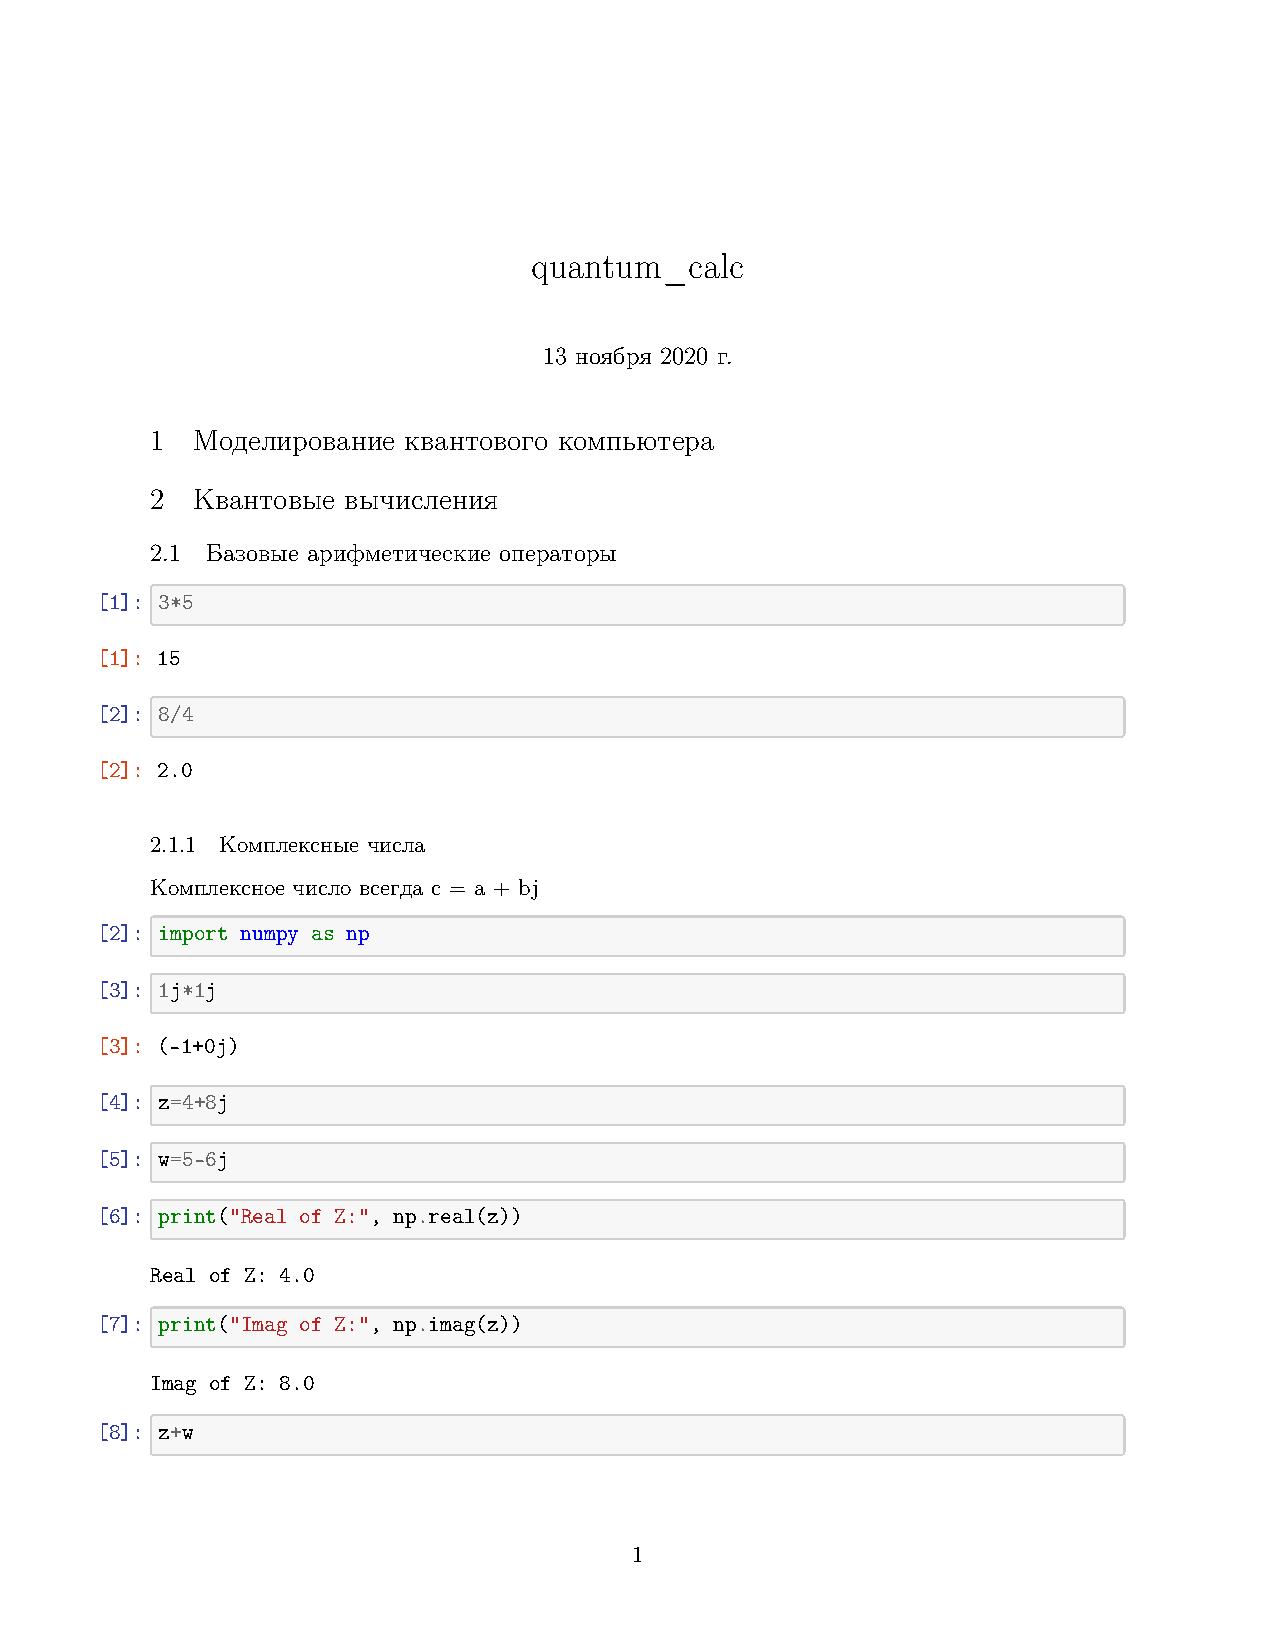
\includepdf[page={1-14}]{quantum_calc}

\section{Заключение}
В статье было продемонстрирована легкость разрабатки квантового алгоритма, возможность проводить численные квантовые эксперименты и запускать их на симуляторах и реальных квантовых компьютерах при использовании Qiskit. В отличии от реализаций на языках программирования, фреймворк предоставляет абстрактный уровень для интеграции с квантовыми компьютерами и их симуляторами, тем самы, является является удобным фронтендом в исследовании квантовых компьютеров и квантовых алгоритмов. Также, к неоспоримым преимуществам относятся возможности визуализации на любом из алгоритмических этапов.

В ноябре был анонсирован CAD система по хардварному моделированию квантовых устройств от концепта до реализации:

\begin{figure}[htp]
\centering
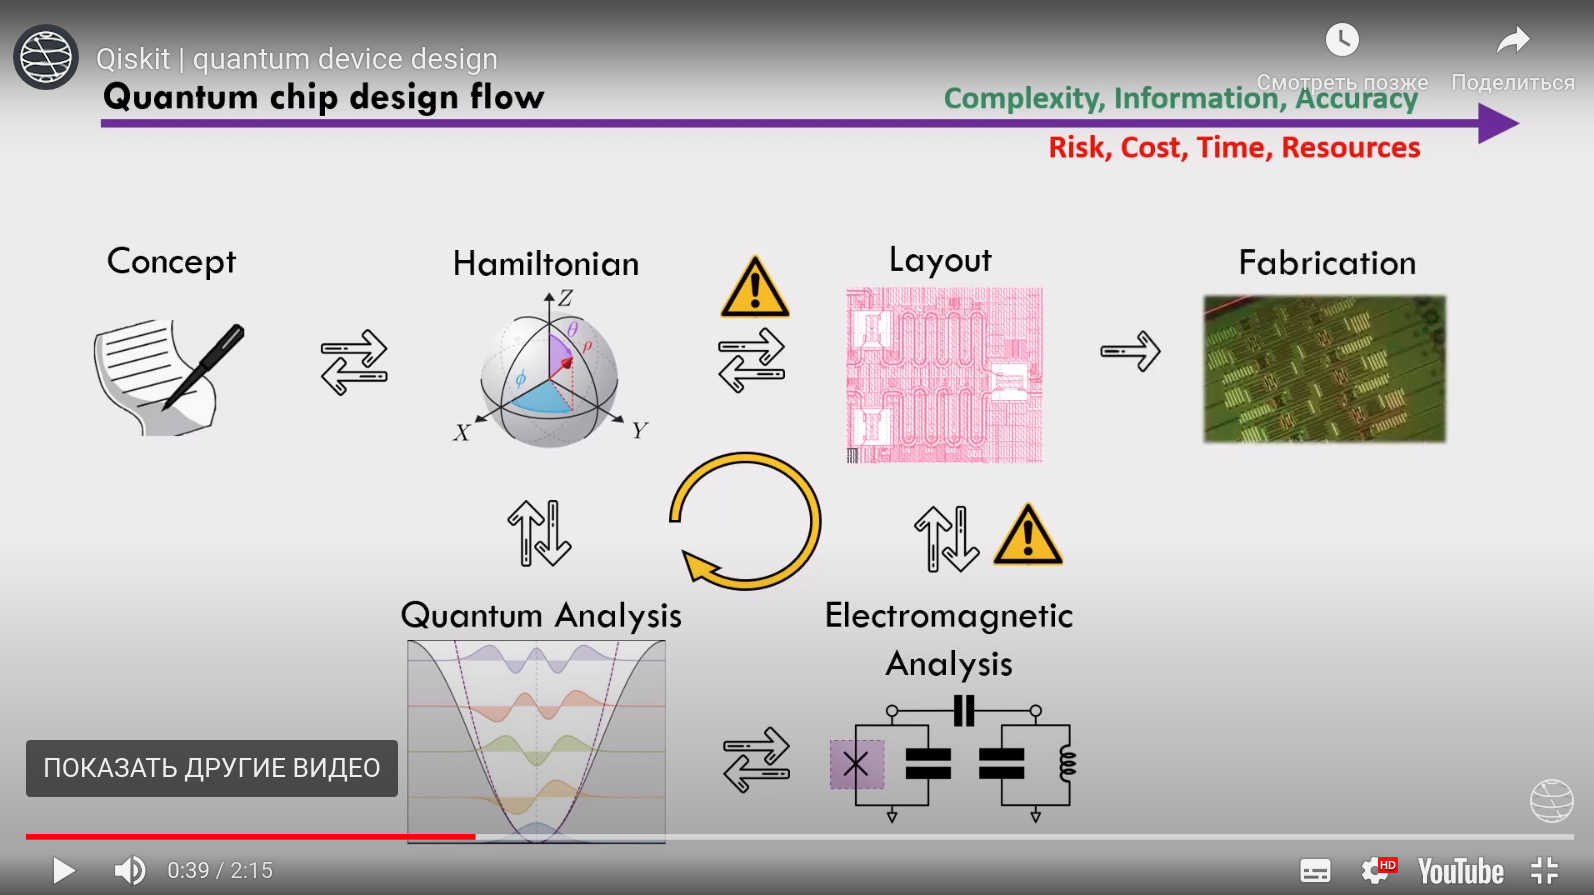
\includegraphics[scale=0.2]{qiskit_1}
\caption{Qiskit этапы проектирования}
\label{}
\end{figure}

Позволяет проектировать устройства, выполнять необходимы рассчеты и проверки, производить компановку на подложке.

Поскольку на текущий момент есть только регистрация, без доступа к продукту, то сложно сказать, возможна ли интеграция кастомизированных устройств. Если это будет предусмотрено, то видится перспективным разработка программных квантовых компонентов по открытым API этой CAD.

\begin{figure}[htp]
\centering
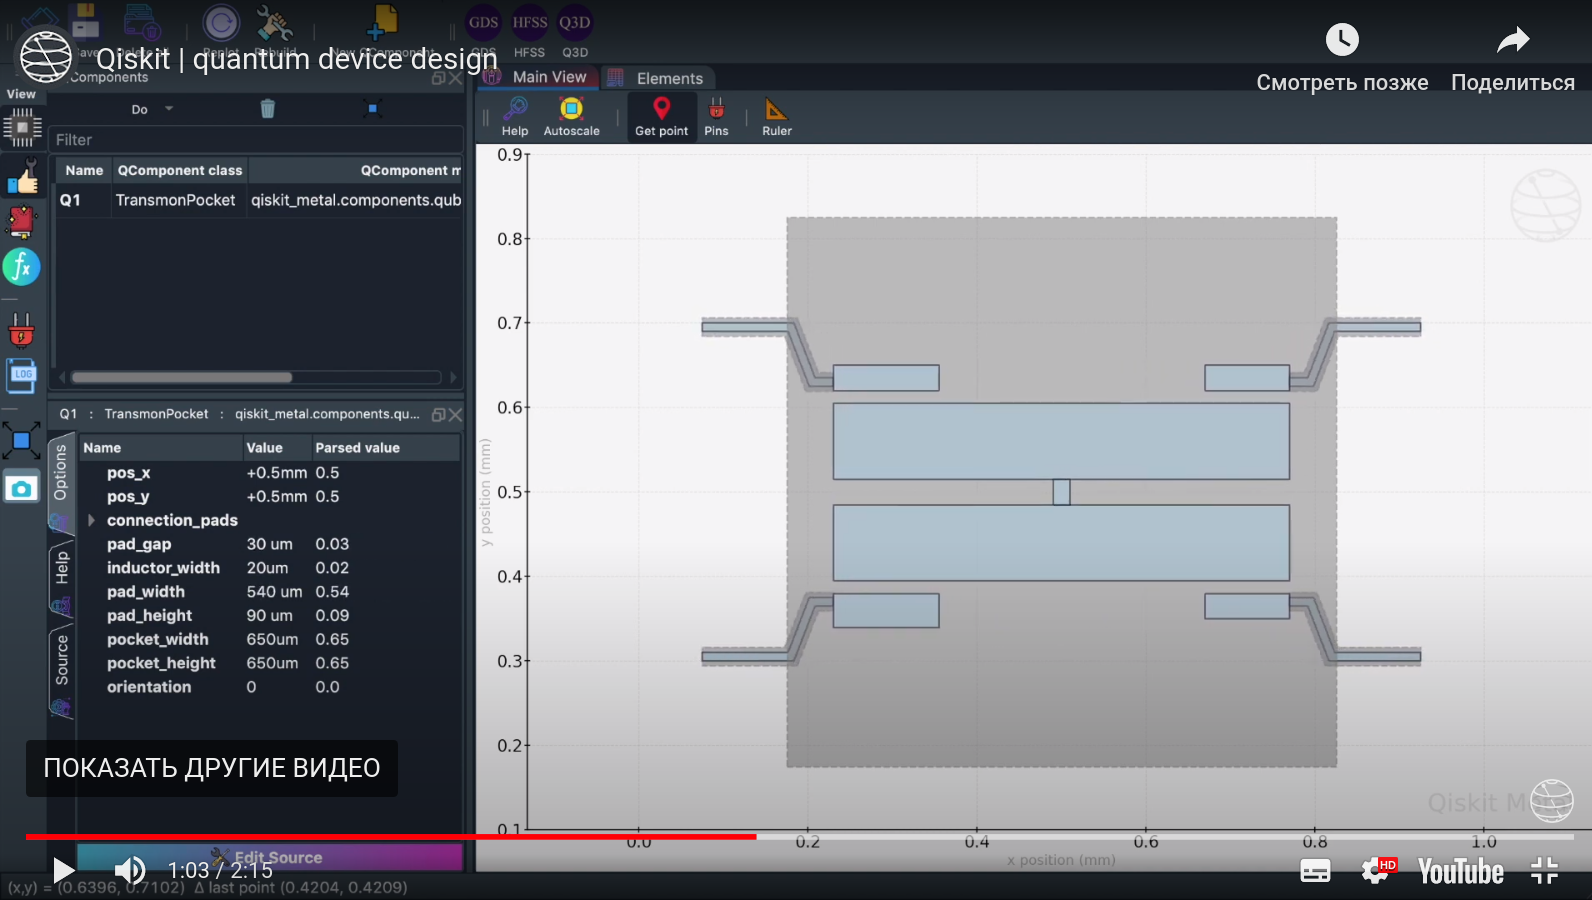
\includegraphics[scale=0.2]{qiskit_2}
\caption{Qiskit проектирование кубита}
\label{}
\end{figure}

\begin{figure}[htp]
\centering
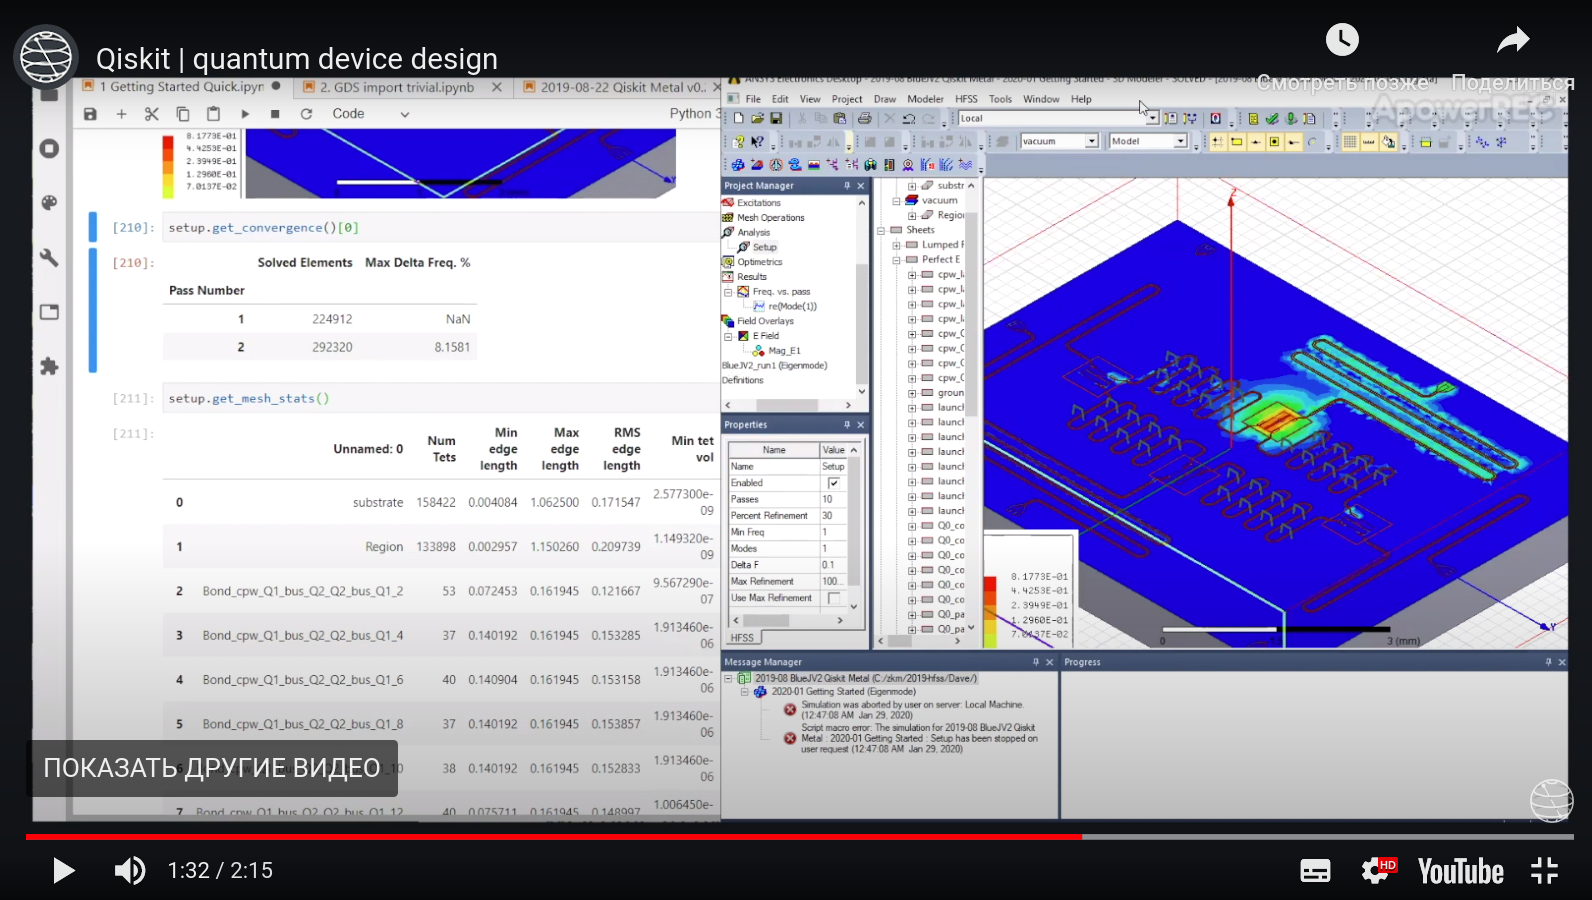
\includegraphics[scale=0.2]{qiskit_3}
\caption{Qiskit 3D-компановка}
\label{}
\end{figure}

\begin{figure}[htp]
\centering
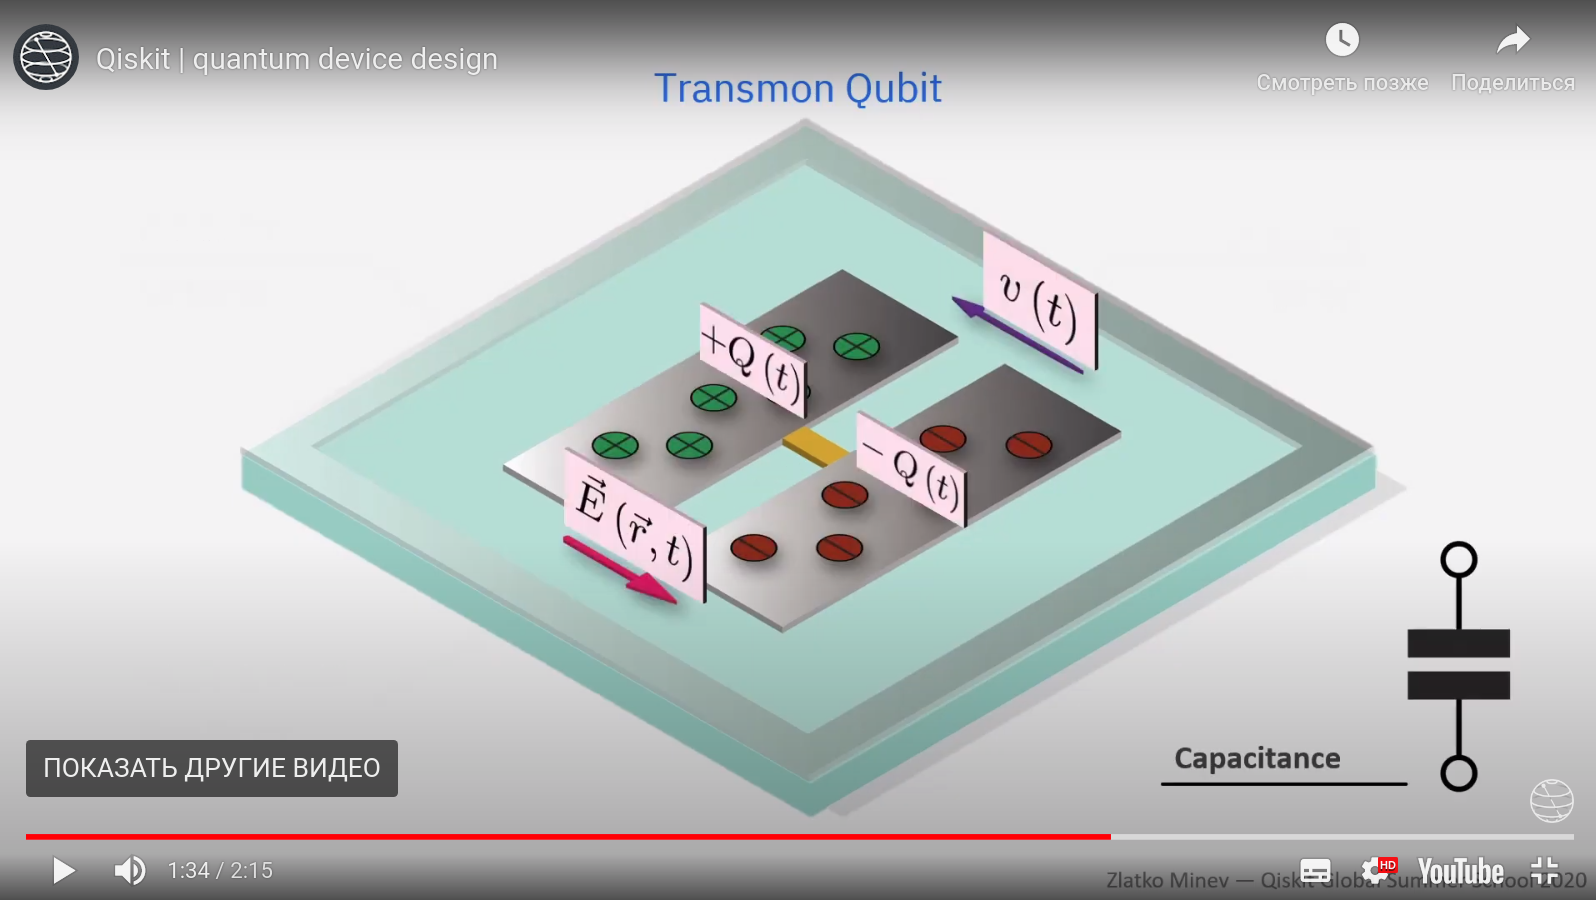
\includegraphics[scale=0.2]{qiskit_4}
\caption{Квантовый анализ конденсатора}
\label{}
\end{figure}

\begin{figure}[htp]
\centering
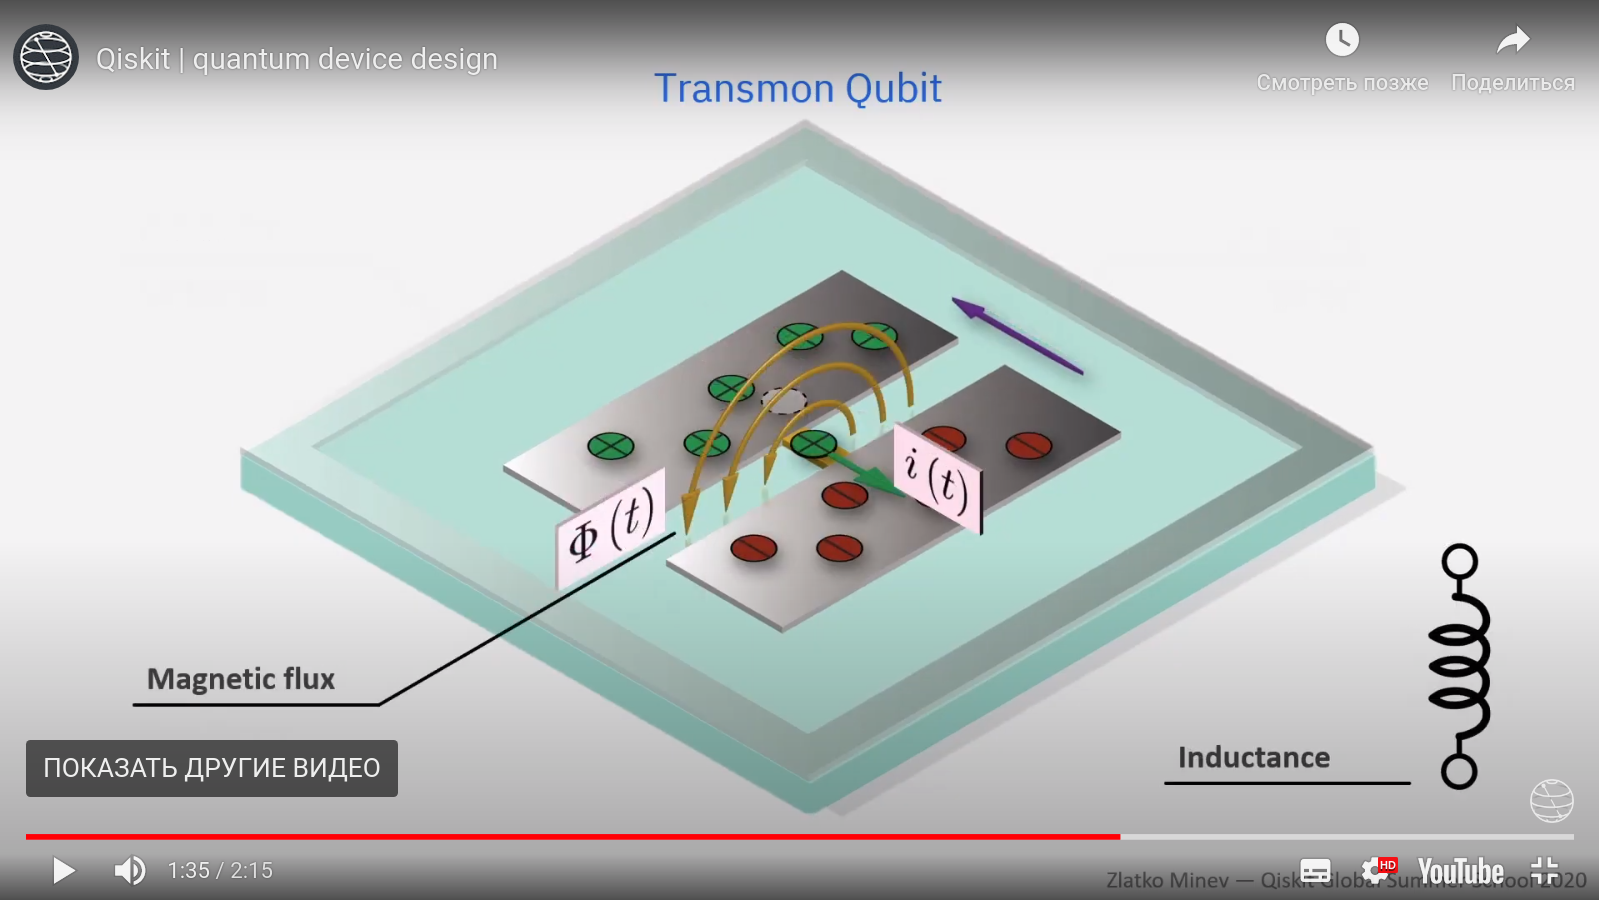
\includegraphics[scale=0.2]{qiskit_5}
\caption{Квантовый анализ индуктивности}
\label{}
\end{figure}

\begin{figure}[htp]
\centering
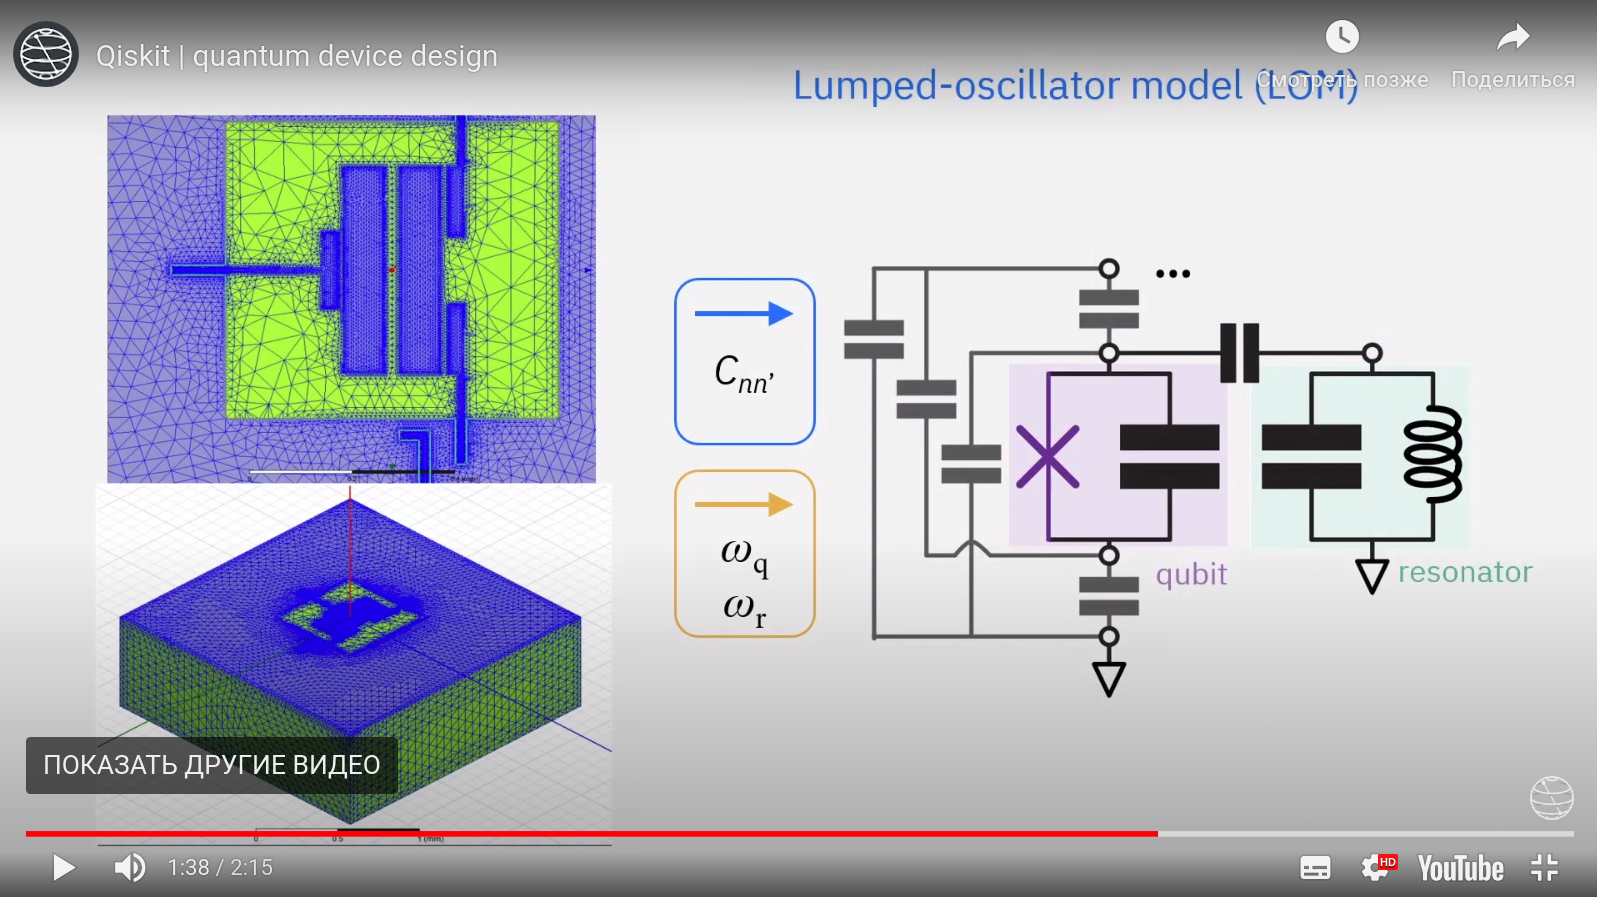
\includegraphics[scale=0.2]{qiskit_6}
\caption{Принципиальное моделирование систем}
\label{}
\end{figure}

\begin{figure}[htp]
\centering
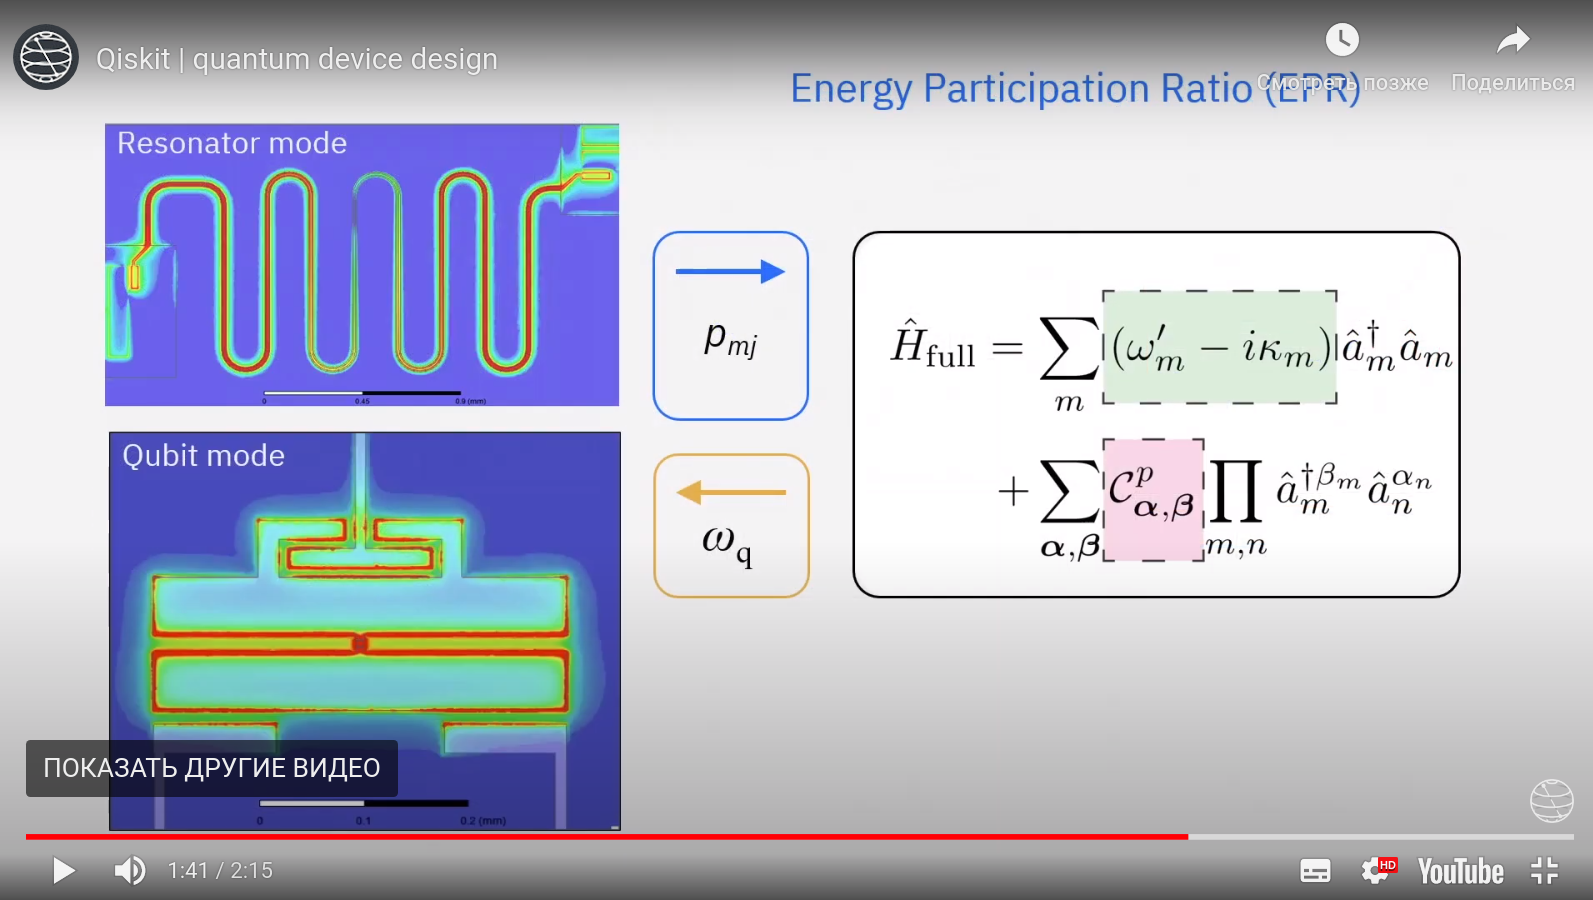
\includegraphics[scale=0.2]{qiskit_7}
\caption{Квантомеханический расчет систем}
\label{}
\end{figure}

В заключении определим место проводимого исследования в современнном технологическом мире - это рисунки 6 и 7 - построение квантовых устройств с использованием ионизирующего излучения.

\begin{thebibliography}{3}

\bibitem{qiskit}
QISKIT 0.23.1 DOCUMENTATION ~\url{https://qiskit.org/documentation/}

\bibitem{jupyter}
Jupiter ~\url{https://jupyter.org/}

\bibitem{hidary}
Hidary, J. D. (2019). Quantum Computing: An Applied Approach. doi:~\url{https://doi.org/10.1007/978-3-030-23922-0} 

\bibitem{coles}
Patrick J. Coles, Stephan Eidenbenz, Scott Pakin, Adetokunbo Adedoyin, John Ambrosiano. Quantum Algorithm Implementations for Beginners // arXiv:1804.03719 [quant-ph]. — 2018.

\bibitem{qiskit_metall}
QISKIT METAL ~\url{https://qiskit.org/metal}

\end{thebibliography}

\end{document}